\documentclass[10pt,a4paper,twoside, twocolumn]{report}
%% Lots of packages !
\usepackage{etex}

%% Francisation
\usepackage[francais]{babel}
\usepackage[T1]{fontenc}
\usepackage[utf8]{inputenc}
%\usepackage{textcomp}

%% Réglages généraux
\usepackage[left=1.5cm,right=1.5cm,top=2cm,bottom=2cm]{geometry}
\usepackage{fancyhdr}
\usepackage{setspace}
\usepackage{lscape}
%\usepackage{multicol}
\usepackage{makeidx}
\usepackage[clearempty]{titlesec}
\usepackage{cite}

%% Packages pour le texte
\usepackage{pifont}
\usepackage{eurosym}
\usepackage{soul}
\usepackage[normalem]{ulem}
\usepackage{fancybox}
\usepackage{boxedminipage}
\usepackage{enumerate}
\usepackage{verbatim}
\usepackage{moreverb}
\usepackage{listings}
\usepackage[table]{xcolor}

%% Packages pour les tableaux
\usepackage{array}
\usepackage{multirow}
\usepackage{tabularx}
\usepackage{longtable}

%% Packages pour les dessins
\usepackage{graphicx}
\usepackage{wrapfig}
%\usepackage{picins}
\usepackage{picinpar}
\usepackage{epic}
\usepackage{eepic}
\usepackage{tikz}
\usepackage{afterpage}
\usepackage{rotating}
\usepackage{float}
\usepackage{caption}

%% Packages pour les maths
\usepackage{amsmath}
\usepackage{amssymb}
\usepackage{dsfont}
\usepackage{mathrsfs}
\usepackage{bussproofs}
\usepackage[thmmarks,amsmath]{ntheorem}

%% Création de nouvelles commandes
%\usepackage{calc}
\usepackage{ifthen}
\usepackage{xspace}



\usepackage{url}
\usepackage{hyperref}
\usepackage{todonotes}
\usepackage{subcaption}
\usepackage[french,ruled,vlined,linesnumbered,algochapter,dotocloa]{algorithm2e}
\usepackage{MnSymbol}

\usepackage{chngcntr}

\usepackage{standalone}
\usepackage{import}



\frenchbsetup{StandardEnumerateEnv=true}

%% =======================================================================

\fancypagestyle{empty}{%
  \fancyhf{}
  \fancyhead[L]{}
  \fancyhead[C]{}
  \fancyhead[R]{}
  \fancyfoot[L]{}
  \fancyfoot[C]{}
  \fancyfoot[R]{}
}
\fancypagestyle{basicstyle}{
	\fancyhf{}	
	\fancyhead[L]{}
	\fancyhead[C]{Rendu réaliste et temps réel pour la réalité augmentée}
	\fancyhead[R]{}
	\fancyfoot[L]{hadrien.croubois@ens-lyon.fr}
	\fancyfoot[C]{--~\thepage~--}
	\fancyfoot[R]{}
}
\pagestyle{basicstyle}

%% =======================================================================

\titleformat{\section}[frame]
{\normalfont}
{\filright \footnotesize \enspace Partie \thesection\enspace}
{6pt}
{\bfseries\filcenter}
	
\titleformat{\subsection}[frame]
{\normalfont}
{\filright \footnotesize \enspace \thesubsection\enspace}
{6pt}
{\filcenter}

\titleformat{\subsubsection}
{\titlerule \vspace{.8ex} \normalfont\itshape}
{\thesubsubsection}
{.5em}
{}

\titleformat{\chapter}[display]
{\normalfont\bfseries\filcenter}
{}
{1ex}
{\titlerule[2pt] \vspace{2ex} \LARGE}
[\vspace{1ex} {\titlerule[2pt]}]

\parindent=10pt
\DeclareUnicodeCharacter{00A0}{~}

%% =======================================================================



\newcommand{\HRule}{\rule{\linewidth}{0.5mm}}
\newcommand{\Hs}{\operatorname{HS}}




\floatstyle{ruled}
\restylefloat{figure}
\restylefloat{table}
\newfloat{code}{!h}{locode}{}
\floatname{code}{\textsc{code}}

\addto\captionsfrench{%
  \renewcommand{\listfigurename}{Liste des figures}%
  \renewcommand{\listtablename}{Liste des tableaux}%
  \renewcommand{\listalgorithmcfname}{Liste des algorithmes}%
}
\newcommand{\listofcode}{\listof{code}{Liste des codes}}

\numberwithin{code}{chapter}
\numberwithin{equation}{subsection}
\counterwithout{footnote}{chapter}






\newcommand{\framedgraphics}[2]{%
  \setlength{\fboxsep}{0pt}%
  \setlength{\fboxrule}{1pt}%
  \fbox{\includegraphics[{#1}]{{#2}}}%
}

\newcommand*{\captionsource}[2]{%
  \caption[{#1}]{%
    #1%
    \\\hspace{\linewidth}%
    \textbf{\textsc{Source}} #2%
  }%
}

\newcommand{\footurl}[2][]{\footnote{\textbf{#1}\href{#2}{#2}}}
% \newcommand{\footurl}[2][]{\footnote{\textbf{#1}\url{#2}}}







\newif\iftwocolumn
\twocolumntrue
\usetikzlibrary{3d,arrows, calc, backgrounds, petri, positioning, shadows, shapes}


\tikzset{
	persp/.style={scale=3.0,x={(-0.8cm,-0.4cm)},y={(0.8cm,-0.4cm)}, z={(0cm,1cm)}},
	points/.style={fill=white,draw=black,thick}
	grid/.style={very thin,gray},
	axis/.style={->,ultra thick},
	cube/.style={thick, fill=black!15,opacity=0.5},
	cube hidden/.style={dashed},
	block/.style={
		rectangle, rounded corners,
		draw=black!80,
		fill=black!10, fill opacity=0.5,
		text=black!90, text opacity=1.0,
    text height=1.5ex,
    text depth=.25ex,
    text width=6em,
    text centered
	}
}

\tikzstyle{class}			=[rectangle, rounded corners, draw=black, fill=blue!40, drop shadow, text centered, anchor=north, text=white,    text width=3cm]
\tikzstyle{module}		=[rectangle, rounded corners, draw=black, fill=red!40, 	drop shadow, text centered, anchor=north, text=white,    text width=3cm]
\tikzstyle{component}	=[rectangle, rounded corners, draw=black, fill=green,   drop shadow, text centered, anchor=north, text=black!90, text width=3cm]
\tikzstyle{single}		=[text height=1.5ex, text depth=0.25ex]
\tikzstyle{double}		=[text height=4.0ex, text depth=2.75ex]
\tikzstyle{triple}		=[text height=6.5ex, text depth=5.25ex]
\tikzstyle{quadru}		=[text height=9.0ex, text depth=7.75ex]
\newcommand*{\rootPath}{../}
\standalonetrue

\begin{document}


\iftwocolumn \twocolumn \else \onecolumn \fi


\chapter{Repérage dans l’espace}

Afin de pouvoir proceder à l'integration d'un objet dans une scène, il est necessaire de pouvoir positionner le périphérique d'acquisition par rapport à la scène. Ces informations de positionnement sont necessaires non seulement au positionnement de l'objet virtuel mais également à la reconstruction de l'evironnement lumineux.

\section{Hiérarchie de référentiels}

Afin de mettre en place les différents mécanismes de repérage, il a été nécessaire de hiérarchiser les repères relatifs aux différents référentiels considérés.

Le référentiel principal est le référentiel du monde. Il est par définition fixe au cours du temps et est défini par rapport à la mire utilisée pour l’acquisition. Ce repère est placé au centre géométrique de la mire et servira aussi bien à positionner l’objet à afficher qu’à définir le référentiel de base pour l’envmap.

Les différentes faces de la mire sont elles-mêmes fixes dans le repère du monde car liées à l’objet physique (la mire) qui le défini. Les transformations entre le repère de chacune des faces de la mire et le repère du monde sont codées dans les marqueurs présents sur les faces (matrice $model$).

Ainsi, ayant identifié une des faces à l’aide du marqueur présent sur cette dernière, il est possible, en appliquant la transformation codée par ce marqueur, de reconstruire le repère du monde.

L’interface d’acquisition est elle aussi positionnée vis-à-vis du repère principal. La transformation entre ces deux repères est codée par la matrice $view$ et changera au cours du temps, l’utilisateur se déplaçant par rapport à la mire.

\begin{figure}[!ht]
	\centering
	\includestandalone[width=0.4\textwidth]{\rootPath Figures/spaceHierarchie}
	\caption{Les différents référentiels}
	\label{fig:tikz:spaceHierarchie}
\end{figure}

Les différentes caméras présentes sur l’interface d’acquisition seront à leur tour positionnées relativement à l’interface d’acquisition. Cette dernière transformation est disponible dans les fichiers de configuration de caméra chargés au démarrage.

\begin{table}[!ht]
	\centering
	\begin{tabular}{rcl}
																			& \textbf{QRcode}				&																\\[.2cm]
		$ $																& $\updownharpoons$			& $ $														\\[.2cm]
																			& \textbf{Face}					&																\\[.2cm]
		$model^{-1}				\lcurvearrowup$	&												& $\lcurvearrowdown model$			\\[.2cm]
																			& \textbf{Monde}				&																\\[.2cm]
		$view^{-1}				\lcurvearrowup$	& 											& $\lcurvearrowdown view$				\\[.2cm]
																			& \textbf{Smartphone}		&																\\[.2cm]
		$orientation^{-1}	\lcurvearrowup$	& 											& $\lcurvearrowdown orientation$\\[.2cm]
																			& \textbf{Caméra}				&																\\[.2cm]
		$cvToGl^{-1}			\lcurvearrowup$	& 											& $\lcurvearrowdown cvToGl $		\\[.2cm]
																			& \textbf{Vue OpenGL}		&																\\[.2cm]
		$projection^{-1}	\lcurvearrowup$	&												& $\lcurvearrowdown projection$	\\[.2cm]
																			& \textbf{Image rendue}	&
	\end{tabular}
	\caption{Hiérarchie des matrices de transformations}
	\label{ref:table:hierarchie}
\end{table}



\section{Utilisation de marqueurs}

L’évaluation des transformations, qui est nécessaire au positionnement dans la scène et donc à la reconstruction de l’environnement, nécessite la reconnaissance de marqueurs. L’identification de ces marqueurs, fixes dans l’espace du monde, associée à la connaissance de la matrice $model$ correspondante permettent de calculer l’orientation au regard de la scène.

Afin de maximiser la reconnaissance de la scène dans sa globalité, il est nécessaire de construire une mire complète, disposant de plusieurs faces parmi lesquelles au moins une devra, pour toute orientation, être lisible. Les marqueurs constituants cette mire doivent par ailleurs être capables de porter les informations caractéristiques de la matrice $model$ associée.

Il est donc nécessaire de choisir un modèle de marqueurs permettant à la fois une localisation précise d’au moins trois points (nécessaires au repérage) et portant des informations propres.

Parmi les nombreux modèles de marqueurs répondant au pré-requis, le choix d’une implémentation s’est rapidement porté sur un modèle utilisant des QR codes\footurl[QRCode:~]{http://www.qrcode.com/}. L’adaptation à un autre modèle est particulièrement aisée puisqu’elle ne demande que le développement d’un module de scanner reconnaissant les marqueurs (voir section~\ref{section:module:scanner}, page~\pageref{section:module:scanner}).

Sont disponibles en annexe les patrons des mires cubiques (figure~\ref{extra:patron_cube}, page~\pageref{extra:patron_cube}) et hémisphériques octogonales (figure~\ref{extra:patron_octo}, page~\pageref{extra:patron_octo}) construites à base de QR codes.



\section{Évaluation des transformations}

Compte tenu de la hiérarchie de référentiel décrite dans la section précédente, il est nécessaire, pour décrire complètement le système, de décrire chacune des matrices de transformation. 


\subsection{Calibrage de la caméra}

L’étape de calibrage de caméra permet de calculer les différents termes de la matrice $projection$ propre à l’interface d’acquisition. Ici l’interface est simplement modélisée suivant le modèle communément admis de sténopé (ce qui revient à assimiler l’objectif à un simple point), dont la calibration détermine les caractéristique physiques (longueur focale, définition du capteur).
%Cela revient à ajuster le modèle de sténopé considéré dans la section~\ref{section:modele} avec les paramètres physiques.

La matrice $projection$ est de la forme suivante :

\begin{equation}
	\begin{pmatrix}
		\alpha_x	&	\gamma		& u_0	\\
		0					&	\alpha_y	&	v_0	\\
		0					&	0					&	1
	\end{pmatrix}
\end{equation}
avec 
\begin{align*}
	\alpha_x	&= f * m_x	\\
	\alpha_y	&= f * m_y
\end{align*}
où $f$ est la longueur focale, $m$ est la résolution du capteur selon les axes $\vec x$ et $\vec y$, $u_0$ et $v_0$ sont les coordonnées du centre optique sur le capteur et $\gamma$ est un coefficient qui décrit la non orthogonalité des axe principaux.

Le calcul de cette matrice est résolu par la minimisation d’un système linéaire sur de nombreuses prises de vue du marqueur. 

Cette étape de calibration est implémentée par la bibliothèque OpenCV\footurl[OpenCV:~]{http://opencv.org/}.

Une fois déterminés, les paramètres relatifs à la caméra sont sauvegardés dans un fichier \texttt{xml}.

\subsection{Positionnement à partir de marqueurs}\label{section:positionnement}

Une fois la caméra calibrée, c’est-à-dire une fois les paramètres intrinsèques déterminés il est possible d’utiliser la connaissance de la matrice $projection$ et des dimensions du marqueur pour reconstruire, à partir des coordonnées du marqueur dans l’espace image, la matrice de transformation $extrinsic$ correspondant au passage de l’espace du QR code (face de la mire) à l’espace de la caméra.

Les matrices $model$ et $orientation$ étant connues, la première grâce aux informations écrites sur le QR code et la seconde étant pré-enregistrée (fixe, liée à la géométrie du téléphone), il est possible d’en déduire la matrice $view$ qui caractérise le positionnement dans la scène :

\begin{align}
	view	&=			orientation^{-1}	\notag \\
%%			&\times cvToGl^{-1}				\notag \\
				&\times extrinsic					\notag \\
				&\times model^{-1}
\end{align}

\subsection{Models OpenCV / OpenGL}

Les différentes bibliothèques ont chacune leurs approches qui inpliquent des différences de conventions.

OpenCV considère les images comme des matrices. À ce titre l’origine est placée en haut à gauche, avec le $\vec x$ pointant vers la gauche et le vecteur $\vec y$ pointant vers le bas. Ainsi regarder une image revient à regarder selon l’axe des $\vec z$ croissants.

% \begin{figure}[!ht]
% 	\centering
% 	\includestandalone[width=0.33\textwidth]{\rootPath Figures/space-opencv}
% 	\caption{Convention d’orientation OpenCV}
% 	\label{fig:tikz:space-opencv}
% \end{figure}

À l’inverse OpenGL s’intéresse à des espaces $3D$ complets et oriente donc naturellement le vecteur $\vec y$ vers le haut. L’utilisateur regarde donc selon l’axe des $\vec z$ décroissants.

% \begin{figure}[!ht]
% 	\centering
% 	\includestandalone[width=0.33\textwidth]{\rootPath Figures/space-opengl}
% 	\caption{Convention d’orientation OpenGL}
% 	\label{fig:tikz:space-opengl}
% \end{figure}

\begin{figure}[!ht]\centering
	\begin{subfigure}[b]{0.22\textwidth}\centering
		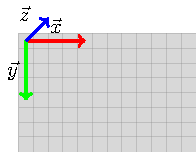
\includegraphics[width=\textwidth]{\rootPath Figures/space-opencv}
		\caption{OpenCV}
	\end{subfigure}
	\begin{subfigure}[b]{0.2\textwidth}\centering
		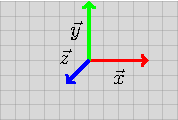
\includegraphics[width=\textwidth]{\rootPath Figures/space-opengl}
		\caption{OpenGL}
	\end{subfigure}

	\caption{Conventions d’orientations}
	\label{fig:tikz:conventions}
\end{figure}


Afin d’utiliser conjointement les deux bibliothèques, il convient de faire les transformations adéquates.

\begin{equation}
	cvToGl = \begin{pmatrix}1 & 0 & 0 \\ 0 & -1 & 0 \\ 0 & 0 & -1\end{pmatrix}
\end{equation}

%=====================================================================
%=====================================================================
\ifstandalone
	\addcontentsline{toc}{chapter}{Bibliographie}
	\bibliographystyle{apalike}
	\bibliography{\rootPath Annexes/biblio}
\fi
%=====================================================================
%=====================================================================
\end{document}